\chapter[The CMS experiment]{The CMS experiment}
\label{chap:CMSExp}
%During the Run II, the Large Hadron Collider (LHC) has produced 
%produced proton-proton collisions at an unprecedented ~\centermassenergy, 
%and at a high luminosity never reached before for 
The CMS and ATLAS experiments are the biggest multi-purpose particle detectors
ever built in the world and  are part of the LHC \cite{chp2:LHCTDR}. The LHC is a 
proton collider located at the CERN laboratory in Switzerland. The 
unprecedented \centermassenergy~of the proton-proton collisions 
produced by this accelerator and its very high luminosity, make possible the search
for physics BSM in a new kinematic regime. The data used for this dissertation comes from
pp collisions produced by the LHC at \sqrts 13 \TeV, and recorded by the CMS experiment during 2016.
In the present Chapter, the LHC accelerator and the CMS experiment will be
described, making emphasis on the CMS subdetectors involved in the 
tau-lepton detection, which plays an important role in this work. 

%This Chapter is organized as follows: First, a brief description of the LHC accelerator is presented;
%next, the CMS subdetector and its subdetectors are described; and finally, the chapter finishes with a brief 
%description of physic objects reconstructed by CMS

\section{LHC Accelerator}
\label{sec:LHC}
The LHC is a particle accelerator designed to collide protons (or lead ions) at 
a \centermassenergy~up to 14 \TeV. The LHC accelerates protons along 
two rings with a circumference of 27 km, installed in a tunnel 
approximately 100 m underground. Bunches of protons (or ions)
are accelerated in opposite directions using ratio frequency (RF) cavities along the rings. They 
collide in four different points, where dedicated experiments are placed 
in order to detect the products of the collisions. The four experiments
are: CMS \cite{chp2:CMSTDR,chp2:CMSTDR2}, 
ATLAS \cite{chp2:ATLASTDR}, LHCb \cite{chp2:LHCb} and  ALICE \cite{chp2:ALICETDR} (see Figure \ref{figchp2:LHCringsfigure}). CMS 
and ATLAS are multi-purpose detectors, optimized for the discovery of new physics BSM. The aim of the LHCb detector is to study 
the charge-parity (CP) symmetry violation, which has been postulated to explain the origin of matter-antimatter 
asymmetry in our universe. ALICE is specialized in studying the quark-gluon plasma. Besides these experiments, there 
are two additional smaller ones: TOTEM and LHCf. The TOTEM main goal is accurate measurement of total, elastic and diffractive pp
cross sections. LHCf uses the particles emitted forward by collisions in order to simulate
the cosmic rays behavior in controlled conditions. 

\begin{figure}[ht]
\begin{center}
 \scalebox{0.2}{
          %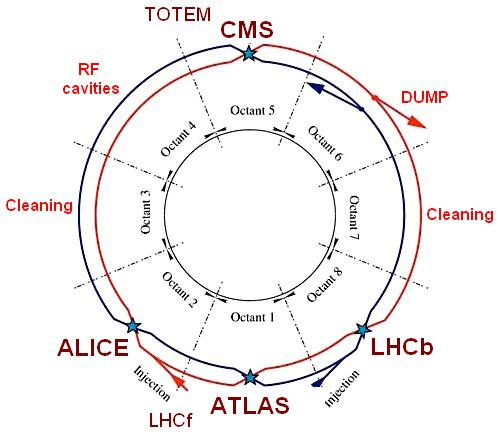
\includegraphics{figuras/Chapter2/LHCrings}}
          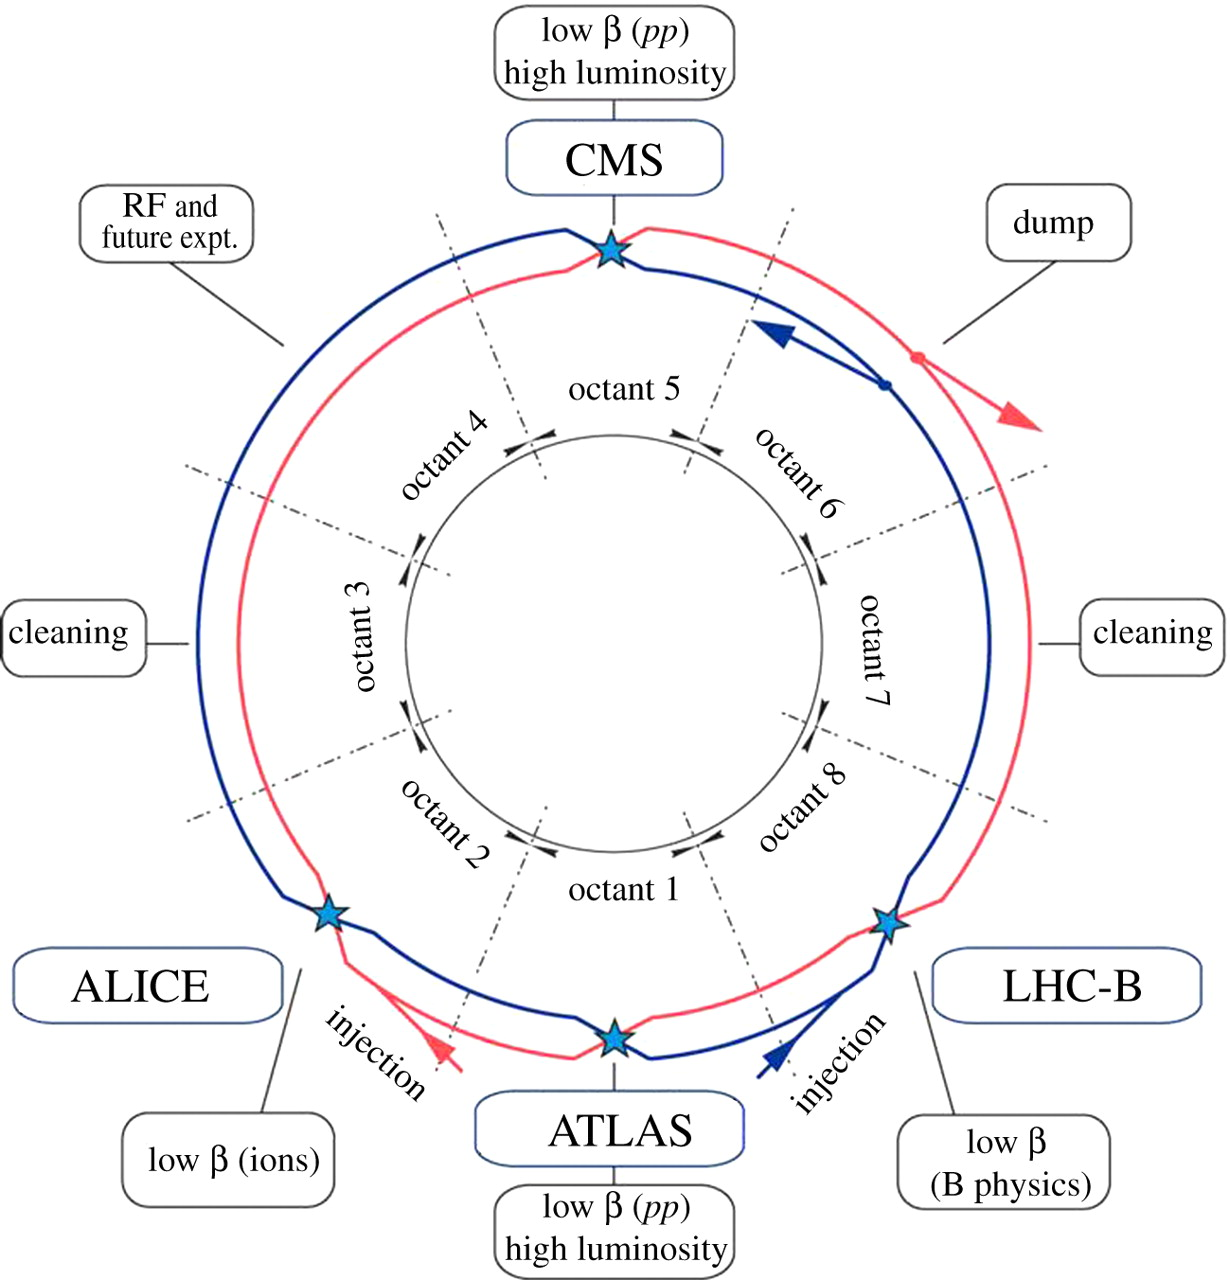
\includegraphics{figuras/Chapter2/LHCrings2}}
\caption{Schematic view of the LHC proton rings showing the interaction points
where the CMS, ATLAS, ALICE and LHCb detectors are located.}\label{figchp2:LHCringsfigure}
\end{center}
\end{figure}

\subsection{LHC Proton Accelerator Chain}
\label{subsec:ProtonAcceleratorChain}

%at an energy of 450 GeV, they have several
In order to achieve the very high energy of the LHC proton beams, several
pre-acceleration stages are used as shown in Figure \ref{figchp2:LHCaccelerationchain}. Before 
protons are injected into the two LHC rings, the process starts 
with the extraction of protons in the \textit{Duoplasmatron 
Proton Ion Source}; in this source, the protons are extracted in ``\textit{bunches}'' 
by ionization of hydrogen gas. Then, these bunches are 
injected into a linear accelerator, \textit{Linac2}, where 
their energy is increased up to 50 \MeV. Once the protons 
reach such energy, they are delivered to the 
\textit{Proton Synchrotron Booster} (PSB) and then to the \textit{Proton Synchrotron} (PS) 
where they are accelerated up to 1.4 \GeV~ and 25 \GeV, respectively. Additionally,
in the PS the bunches are spaced in time by 25 ns\footnote[1]{The time spacing between 
bunches is known as \textit{Bunch Crossing} (BX). For the LHC Run I, the BX was 50 ns; for Run II 
the BX was reduced to its design value of 25 ns.}. The pre-acceleration chain 
finishes in the \textit{Super Proton Synchrotron} (SPS), where the protons reach 
an energy up to 450 \GeV, and then they are injected into the LHC rings. The bunches are 
injected into the LHC rings in opposite directions where they reach an 
energy up to 7 \TeV~per beam; i.e. the LHC could produce proton-proton collisions 
up to 14 \TeV~ in the center-mass frame (\sqrts 14 \TeV). The protons are accelerated 
using 8 RF cavities, which operate with a frequency 
that goes up to 400 MHz in the final acceleration stage and an electric field 
gradient of 5 \MeV~ per meter \cite{chp2:LHCTDR}. The RFs also ensure the longitudinal stability of the beams. The 
proton bunches are radially focused by 392 quadrupole magnets placed along the 
LHC rings. The radial focusing is important to increase the collision probability. Additionally, the 
LHC uses 1232 superconductor dipole magnets, where each of them produce a magnetic field strength 
up to 8.3 T, in order to bend the beam along the circular path. The dipoles 
are cooled by superfluid helium at a temperature of 1.9 K, that also helps to improve the vacuum
inside the beam pipes. 

\begin{figure}[ht]
\begin{center}
 \scalebox{0.35}{
          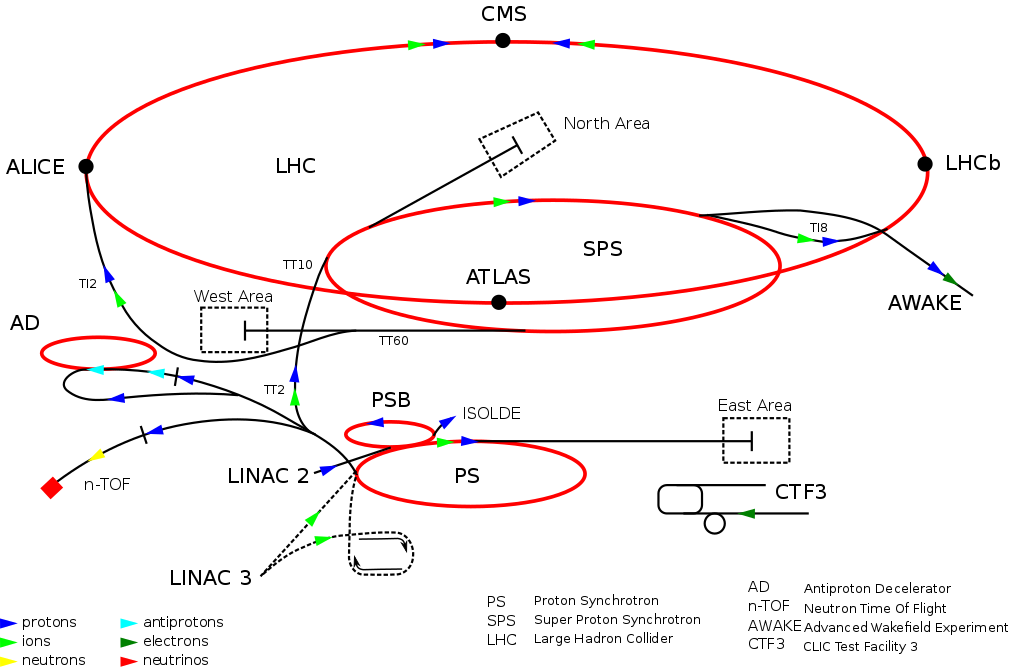
\includegraphics{figuras/Chapter2/LHCaccelerationchain}}
\caption{Schematic view of the proton accelerator chain at CERN.}\label{figchp2:LHCaccelerationchain}
\end{center}
\end{figure}


%since the protons within a bunch will be placed in a smaller cross-section. \\

\subsection{LHC Operational Parameters}
\label{sec:LHCparameters}

The main quantities that describe the performance of a particle accelerator are the beam energy and 
the luminosity. The instantaneous luminosity measures the number of collisions per unit of area 
and per unit of time \footnote[1]{The units of instantaneous luminosity are 
cm$^{-2}$s$^{-1}$.}; it depends on the accelerator's design and, in the 
case of the LHC, it is given by:

\begin{equation}
 L = \frac{N_{b}^{2}k_{b}f_{rev}\gamma}{4 \pi \epsilon \beta^{*}}R \;,
\end{equation}

\noindent where $N_{b}$ is the number of protons per bunch, $k_{b}$ is the number of bunches per beam, $f_{rev}$
is the number of revolutions per second, $\gamma$ is the relativistic factor, $\epsilon$ is the 
normalized transverse beam emittance, $\beta^{*}$ is the optical $\beta$-function at the
collision point and $R$ is a
geometrical factor related with the crossing angle of the two beams. The optimization of 
the instantaneous luminosity is achieved in several ways, such as by increasing the number
of protons per bunch ($N_{b}$) or by increasing the number of bunches per beam ($k_{b}$). For the statistical accuracy 
of the physics measurements, the important quantity is the integrated luminosity \footnote[1]{The units of the 
integrated luminosity are inverse barn, $b^{-1}$.} (instantaneous luminosity integrated in time, $\mathscr{L}$) because the number of events 
produced ($N_{eve}$) is proportional to it, and it is given by the expression:

\begin{equation}
 N_{eve} = \mathscr{L} \sigma_{p} \;,
\end{equation}

\noindent where $\sigma_{p}$ is the cross-section of the process of interest,
for example the cross-section of an hypothetical \Zprime~production, 
$\sigma(pp \rightarrow \textrm{Z}^{\prime})$. If the cross-section that
we want to measure is small, we need a large integrated luminosity
in order to achieve a reasonable number of events, even more, if the process
demands for a complex discrimination between signal and background. For instance, a 
\Zprime~decaying into two taus should have a cross-section of the order of pb, while 
Drell-Yan process, that constitute an important background, has a 
cross-section of around 5780 pb \footnote[7]{In this example, the cross-sections
are estimated for pp collisions at \sqrts 13 \TeV~ and for a \Zprime~with a mass of 500 \GeV.}.
Therefore, the signal discrimination in this case should be of the order of 10$^{-3}$,
demanding even higher luminosities. In addition, in each BX there are several pp
 collisions (of the order of 20, during 2016 data taking period), and only a very small 
 fraction of these collisions correspond to hard proton-proton interactions that could produce
 interesting physics. Most of the collisions correspond to elastic and diffractive scattering
 as well as soft scattering. This means that in a BX with an interesting hard 
 scattering collision there would be another 20 soft scattering ones, that will have to be 
 identified and remove from the event. This phenomenon is known as “pile-up” 
 (PU) and makes difficult the identification of the hard interaction. The level 
 of PU depends on the number of protons per bunch $N_{b}$, as well as on the geometrical 
 factors of the beam. \\
 
\noindent  In order to achieve the high statistics for the identification of BSM signals, a good performance 
 of the LHC accelerator is required. Operational quantities such as beam energy, luminosity, bunch crossing and etc., 
 have been improved from one running period to the next. Table \ref{chp2:LHCtable}
 shows the most relevant quantities of the LHC operation per year.
 
 
\begin{table}[ht]
\begin{center}
\begin{tabular}{|l|c|c|c|c|c|c|} \hline \hline
                                                     &                &                 \multicolumn{3}{|c|}{Run I}            &  \multicolumn{2}{|c|}{Run II}        \\    \cline{3-7}
                                                     &     Design     &       2010      &       2011       &       2012        &       2015       &       2016        \\     \hline \hline   
   Beam Energy [\TeV]                                 &        7       &       3.5       &        3.5       &          4        &        6.5       &        6.5        \\ 
   Number of protons per bunch [10$\times^{11}$]     &      1.15      &       1.0       &        1.3       &        1.5        &        1.1       &        1.1        \\
   Number of bunches per beam                        &      2808      &       368       &       1380       &       1380        &       2244       &       2200        \\
   Bunch Spacing [ns]                                &        25      &       150       &         50       &         50        &         25       &        25         \\
   Average Pile-up in CMS                            &                &                 &                  &         21        &         14       &        27        \\
   Maximum peak luminosity [10$\times^{34}$ cm$^{-2}$s$^{-1}$] & 1.0  &       0.021     &        0.35      &         0.77      &        0.51      &       1.4        \\
   Integrated Luminosity [fb$^{-1}$]                 &                &       0.048     &         5.5      &         22.8      &         4.2      &       40.82       \\  \hline \hline
\end{tabular}
\end{center}
\caption{Some relevant operational parameters for Run II, compared with values reached during Run I \cite{chp2:LHCparameters}.}\label{chp2:LHCtable}
\end{table}

\subsubsection{Run I and Run II of the LHC}
\label{subsubsec:LHCruns}

The LHC operational period spanning from 2010 to 2012 is known as Run I. During 2010, the LHC 
reached pp collisions at \centermassenergy~of 7 \TeV~ and an integrated luminosity of around 
50 pb$^{-1}$. During 2011 with the same \centermassenergy, an integrated luminosity of approximately 
6 fb$^{-1}$ was obtained. For the 2012 run, the energy per beam was increased 
up to 4 \TeV~ (\sqrts 8 \TeV), reaching approximately 20 fb$^{-1}$. The integrated luminosity delivered 
by the LHC and recorded by CMS during Run I is shown in Figure \ref{figchp2:luminosityRunI}. Afterwards, a two-years
technical shut-down took place. \\

\begin{figure}[ht]
    \begin{center}
      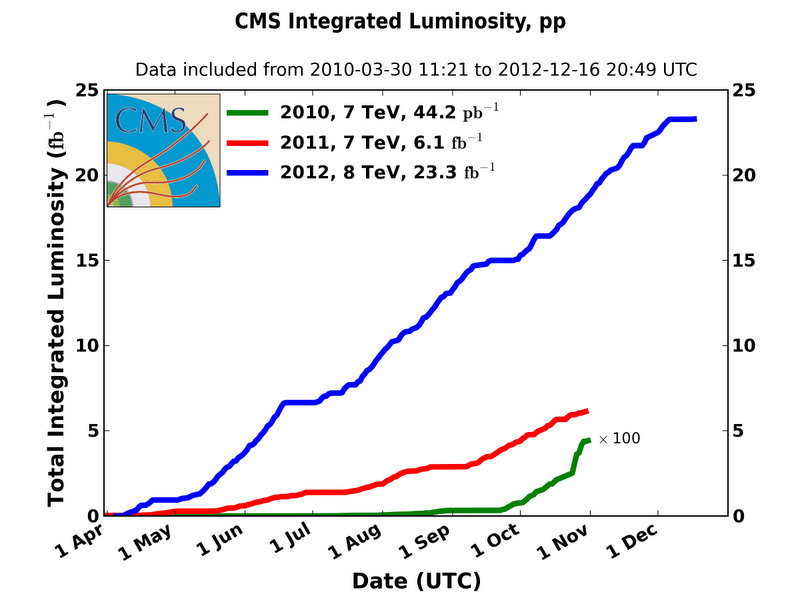
\includegraphics[width=0.5\textwidth]{figuras/Chapter2/CMSluminosityRunI.jpg}
      \caption{CMS integrated luminosity for proton-proton collisions delivered
      in Run I at the LHC. Taken from \cite{chp2:LHCluminosity}.}
     \label{figchp2:luminosityRunI}
    \end{center}
\end{figure}

\noindent After the shut-down, a new data taking period, known as Run II, started on May 
2015. That year, LHC delivered 4.2 fb$^{-1}$ of pp collisions at \sqrts~13 \TeV. During 2016, LHC 
operated at the same \centermassenergy~than during 2015 and reached 40.82 fb$^{-1}$, exceeding  in 53$\%$ the expected integrated 
luminosity ($\sim$26 fb$^{-1}$). The integrated luminosity delivered by the LHC and recorded by CMS, 
during 2015 and 2016, is shown in Figure \ref{figchp2:luminosityRunII}. The success of the 2016 run was due to
the LHC operational stability and the high peak luminosity reached (1.4$\times10^{34}$cm$^{-2}$s$^{-1}$, which represented 
an improvement of 40$\%$ over the design value); this was achieved due to 
the shortening of the beam size from the injectors and the reduction of the 
crossing angle between the two beams. Compared with the 2015 run, the 2016 run 
reduced the number of protons per bunch to 1.1$\times10^{11}$ and the number of bunches per beam 
from 2244 to 2200, keeping the BX at 25 ns. As a result, the average
PU went from 14 in the 2015 run to 27 in the 2016 run (see Table \ref{chp2:LHCtable}). As already mentioned, 
the data used for this dissertation is the one recorded by CMS during 2016 run.
%During this period in order to ensure a good LHC performance for the expected high luminosity and a higher energy per beam. 
\begin{figure}[ht]
    \begin{center}
      \subfloat[2015]{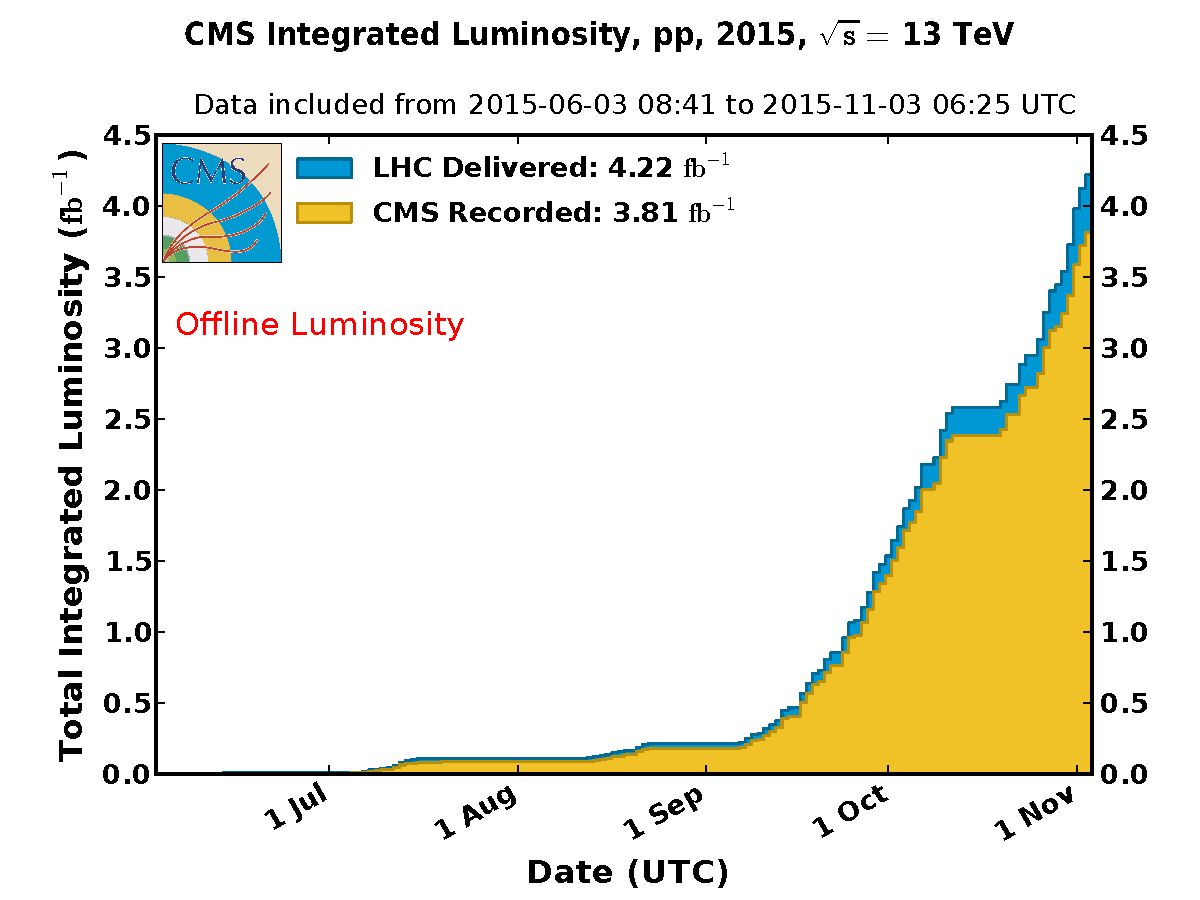
\includegraphics[width=0.5\textwidth]{figuras/Chapter2/CMSluminosity2015.pdf}}
      \subfloat[2016]{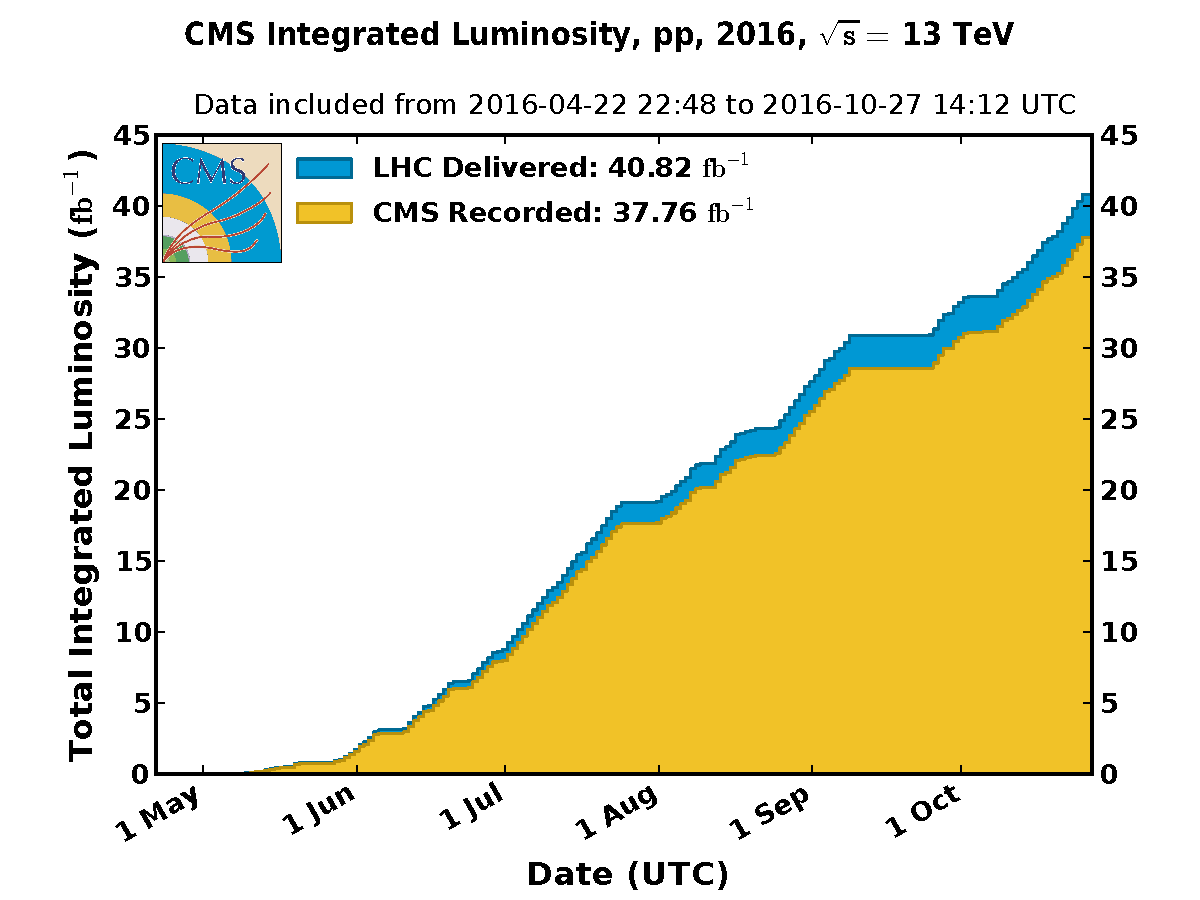
\includegraphics[width=0.5\textwidth]{figuras/Chapter2/CMSluminosity2016.pdf}}
      \caption{CMS integrated luminosity for proton-proton collisions delivered
      in Run II at the LHC. Figures taken from \cite{chp2:LHCluminosity}.}
      %During 2016 LHC delivered 40.82 fb$^{-1}$ and CMS recorded 39.7 fb$^{-1}$. 
     \label{figchp2:luminosityRunII}
    \end{center}
\end{figure}

\section{The CMS Detector}
\label{sec:CMS}

The Compact Muon Solenoid (CMS) is, along with ATLAS, a multi-purpose detector designed 
with a broad physics program, which includes the understanding of the 
electroweak symmetry breaking through the Higgs mechanism, 
and the search for physics BSM, such as SUSY, extra dimensions, etc. The CMS 
detector is located 100 m underground in ``\textit{Point 5}'' of the 
LHC (see Figure \ref{figchp2:LHCringsfigure}). It is a hermetic detector around the collision
point, with a cylindrical shape that has a length of 21.6 m and a diameter of 14.6 m. One of 
the especial features of the detector is the superconducting solenoid which produces an inner magnetic field 
of $3.8$ T (over a volume of 341.7 m$^{3}$). The strong magnetic field bends the tracks 
of the charged particles coming from the interactions, with the purpose of identifying their 
electric charge and to accurately measure their momentum. Besides the solenoid, the detector 
is composed by four subsystems: encased inside the solenoid are the Tracker System, the 
Electromagnetic Calorimeter (ECAL) and the Hadron Calorimeter (HCAL); and outside the 
magnet are the Muon Chambers. The purpose of the Silicon Tracker is to reconstruct 
the collision vertices and the tracks of the charged particles emerging from the 
collision. The Calorimeter system (ECAL and HCAL) allows to measure the energy of hadrons, electrons and 
photons. The Muon Chambers, embedded inside an iron-yoke structure, reconstruct the 
muon tracks and provide an accurate information for their momentum measurement. The overall layout of CMS detector is shown 
in Figure \ref{figchp2:CMSdetectorfigure}. A more detailed description can be found in Ref.~\cite{chp2:CMS}. \\

\begin{figure}[ht]
    \begin{center}
      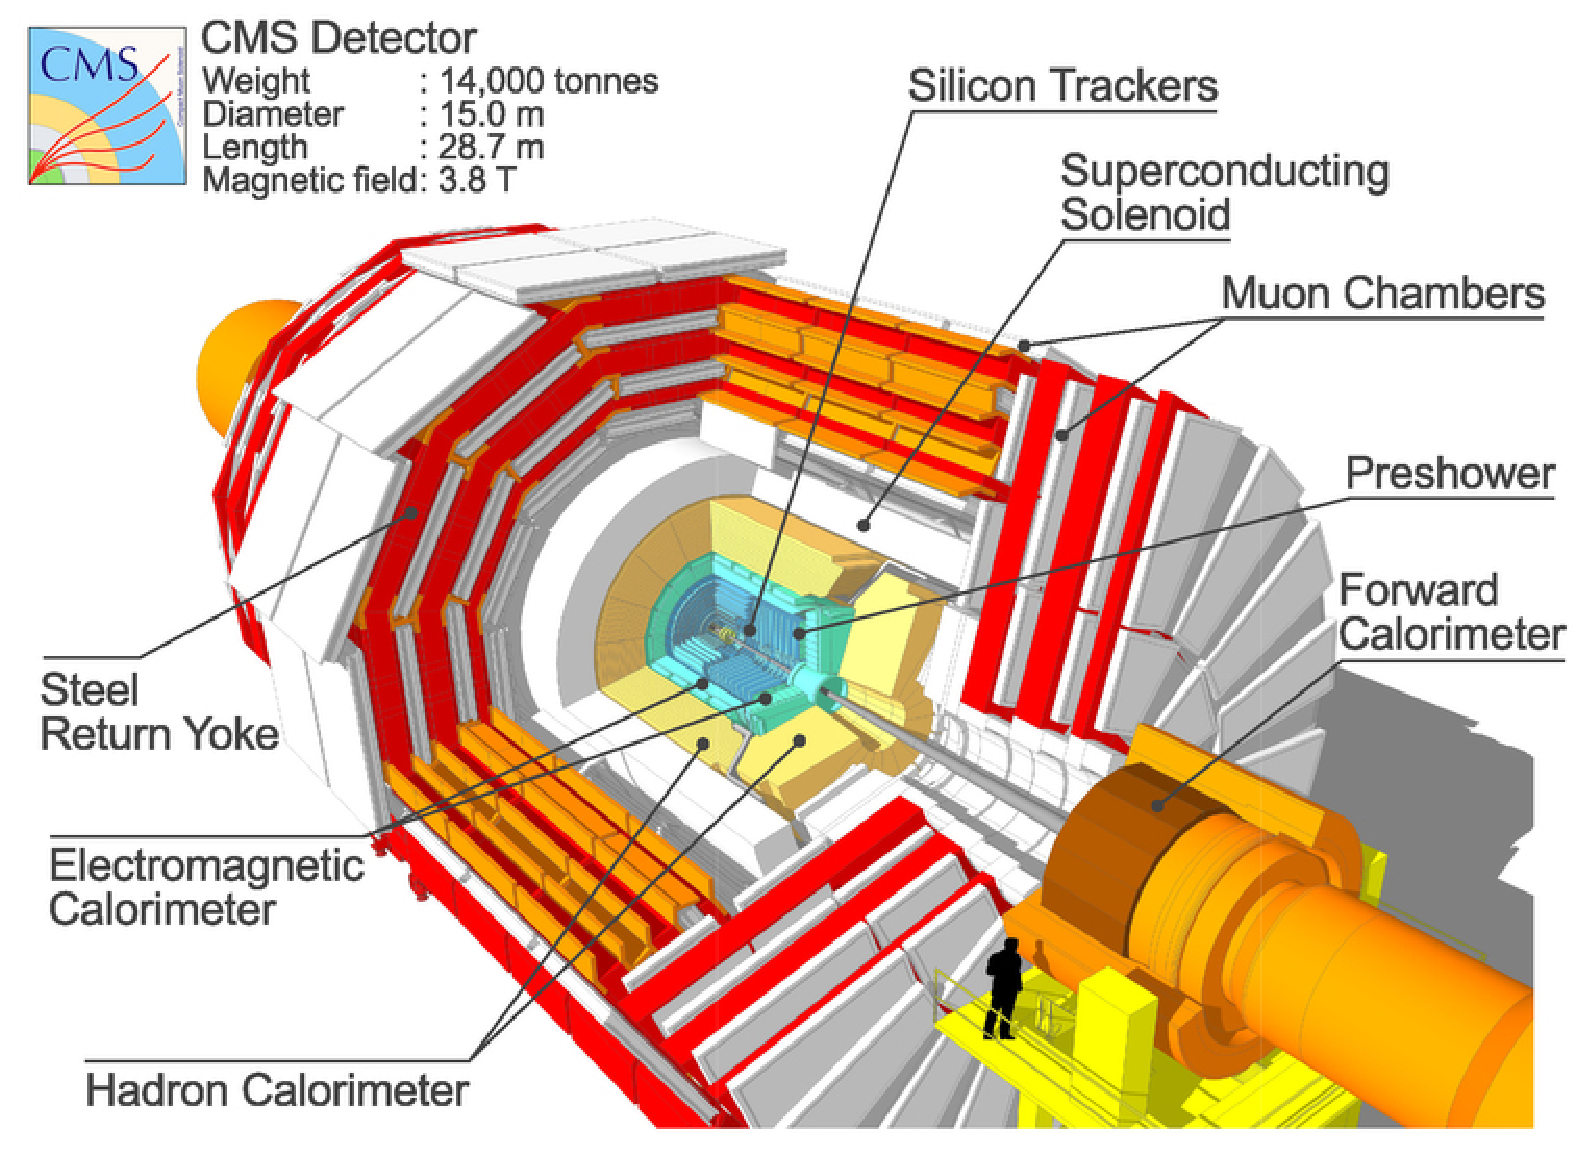
\includegraphics[width=0.7\textwidth]{figuras/Chapter2/CMSdetector.pdf}
       \caption{CMS Detector overview \cite{chp2:CMSTDR}.}\label{figchp2:CMSdetectorfigure}
\end{center}
\end{figure}

\noindent All the information produced in an event is stored in the readout electronics 
of each sub-detector. Once the event information is compressed, the data size
for one bunch crossing is around 1 MB therefore, with the nominal LHC luminosity, CMS would 
produce 40 TB of information per second; this high rate makes impossible 
the data storage with the current technology. Nevertheless, interesting physics can be produced only 
in hard-interaction collisions, which occur approximately once each one million 
collisions. In consequence, CMS uses a Trigger System to select only the hard 
scattering events which are reduced from 40 million collisions per second 
to only 100 events per second, making feasible the data storage. Once the 
Trigger System identifies the interesting events, they are stored in order to be 
analyzed afterward. \\

%PARRAFO HAY QUE MEJORAR TRIGGER Y DAQ Y VOLUMEN DEL SOLENOIDE
%The high collision rate that the LHC produces makes the data storage impossible 
%with the current technology. In consequence, CMS uses a Trigger System to select 
%only the hard scattering events, which are the most likely to have some interesting 
%physics. From 40 million collision per second produced by the LHC, the Trigger 
%System selects and stores only 100 events per second. \\

\textbf{Coordinate System}\\

%CMS is divided into divided into a barrel (central region) and two endcaps.
%In order to locate in space not only the detector components but also the reconstructed
%particles CMS has defined a coordinate system. 

\noindent In order to define the position of any detector components and, in consequence,
of any particle signal, CMS has defined a cartesian and spherical 
coordinate systems. The origin of both systems is the nominal interaction point, which is at the center
of the detector. The x-axis points towards the center of the LHC ring,
the y-axis points upwards and the z-axis points along the beam pipe in the
counterclockwise direction. The polar angle $\theta$ and azimuthal angle $\phi$ are defined 
in the usual way. \\

\noindent In order to parametrize the direction in which the particles are emitted,
the pseudorapidity $\eta$ is better than $\theta$ because its distribution
is more uniform. Pseudorapidity is given by:

\begin{equation}
 \eta = -ln \left( tan \left(\frac{\theta}{2} \right) \right)
\end{equation}

%characterize the is measured from the x-axis in the transverse plane to the beam (x-y plane), while the 
%polar angle $\theta$ is measured from z-axis. %, the polar coordinate used is The pseudorapidity $\eta$ of the particles is related to the polar angle
%instead of $\theta$ %because the distribution of particles is more uniform for $\eta$ than $\theta$. 

\noindent A more detailed description of the CMS coordinate system can be 
found in Ref.~\cite{chp2:CMS}. 

\section{Superconducting Solenoid}
\label{sec:Solenoid}

\noindent The superconducting solenoid produces a uniform inner magnetic 
field with the value of 3.8 T. In the outer region, the 
returning magnetic flux is compactified by the iron yoke, resulting 
on an average magnetic field strength of 2 T. The magnetic field 
provided by the solenoid bends the tracks of the charged particles 
emerging from the collisions (see Figure \ref{figchp2:CMStrajectories}) which is crucial
for their charge identification and their momentum measurement. The electric charge 
is identified according to the direction of the
bending in the magnetic field. The momentum of a charged particle 
that moves through a uniform magnetic field is given by:

\begin{equation}
p = \gamma m v = qBr \;, 
\end{equation}

\noindent where $\gamma$ is the relativistic factor; $m$, $v$, $q$ are its mass,
rapidity and charge, respectively; $B$ is the magnetic field strength; and $r$ is the ratio 
of the bending. A strong magnetic field is necessary for the momentum 
measurement of very energetic charged particles, in consequence the momentum resolution 
depends on the magnetic field strength and the spatial resolution of the detectors 
that reconstruct the tracks. The momentum resolution is:

\begin{equation}
 \frac{\sigma_{p}}{p} \propto \frac{p}{BL^{2}} \;,
\end{equation}

\noindent where $L$ is the length of the trajectory. The strong magnetic field provided by the solenoid 
and the high spatial resolution of the tracker detectors, allows CMS to have 
a very good momentum resolution; for instance, the momentum resolution for muons 
is 1$\%$ up to 100 \GeV~\cite{chp2:CMSTDR2}.\\

%Figure  shows the 
%trajectories for several particles in the solenoid magnetic field.

\begin{figure}[ht]
    \begin{center}
      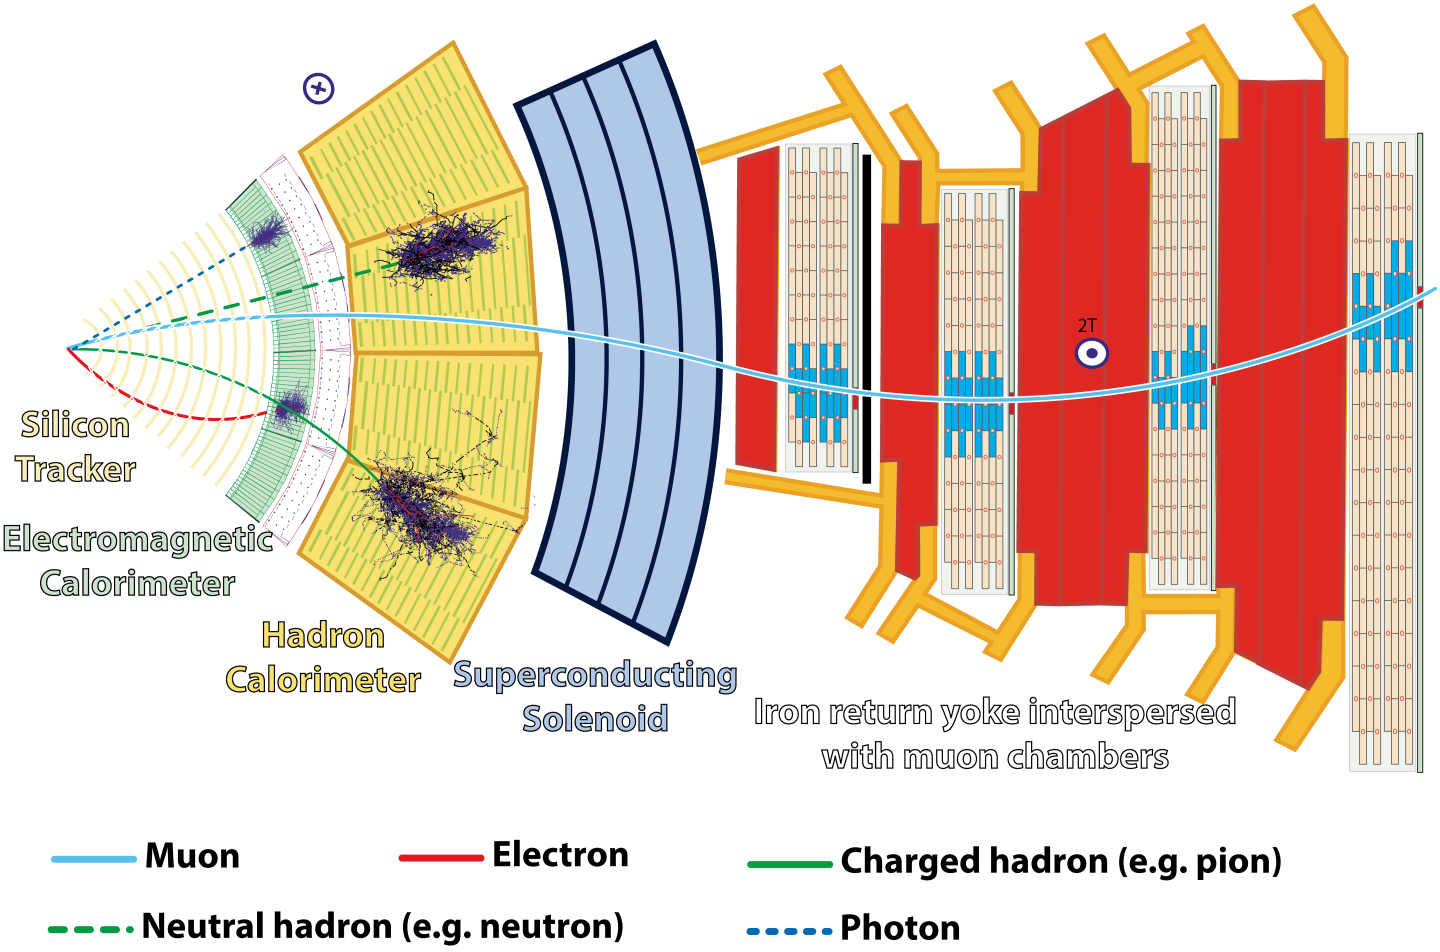
\includegraphics[width=0.7\textwidth]{figuras/Chapter2/CMStrajectories.png}
      \caption{Schematic view on CMS transverse plane for trajectories and energy deposits of several 
      particles moving through the solenoid magnetic field. Taken from \cite{Barney:2120661}.
      } \label{figchp2:CMStrajectories}
    \end{center}
 \end{figure}

\noindent The CMS superconducting solenoid is the biggest one built ever. The coil is made of NbTi with 4 layers of winding. In order to 
generate the strong magnetic field, this solenoid operates
with a nominal current of 19.5 kA, storing an energy up to 2.6 GJ. A cooling system
keeps its superconducting state using liquid helium at 4.65 K. The 
main parameters of the CMS magnet are summarized in Table \ref{tablechp2:Solenoid}.

\begin{table}[h]
\centering
\begin{tabular}{|l|c|}\hline \hline
\multicolumn{2}{|c|}{Magnet Parameters}  \\ \hline \hline
Inner magnetic field   &  3.8 T  \\ \hline
Diameter               &  5.9 m  \\ \hline
Length                 &  12.5 m  \\ \hline
Nominal Current        &  19.5 kA \\ \hline
Stored Energy          &  2.7 GJ  \\ \hline
Inductance             &  14.2 H  \\ \hline \hline
\end{tabular}
\caption{Main parameters of the CMS Solenoid \cite{chp2:CMSTDR}.} \label{tablechp2:Solenoid}
\end{table}



% Weighting 10000 tonnes, this magnet is 12.5 m long and 6 m diameter. 


\section{The Tracker System}
\label{sec:Tracker}

\noindent The Tracker System is the inner-most detector system in CMS. It has 
a cylindrical shape covering an acceptance range of $|\eta| < $ 2.5. This system is 
designed to reconstruct accurately the charged-particle tracks, which is essential 
for achieving a high momentum resolution as well as for identifying the primary and the 
secondary vertices. Secondary vertices are the evidence of the decay 
of long-lived particles coming out the collision, for instance 
jets originated from b-decays, known as \textit{b-jets}, which have a vertex 
that can be distinguished from the primary vertex. Therefore 
a high resolution of secondary vertex reconstruction is required in order to 
identify b-jets (see Section \ref{sec:bJet}). In this dissertation the 
Tracker System is crucial due to the following reasons:

%for the 
%The Tracker System, 
%besides the identification of primary vertex and the reconstruction of 
%charged-hadron tracks, is important in this dissertation for several reasons:

\begin{itemize}
 \item The searches for heavy resonances in the di-lepton channels require a 
 high momentum resolution for leptons with transverse momentum greater than 1 \TeV. 
 \item Since the tau-leptons can decay into charged hadrons (see Section \ref{sec:Taus}), the 
 reconstruction of these hadrons in the Tracker System is crucial
 for the tau identification and reconstruction. Charged
 hadrons are reconstructed with an efficiency of at least 95$\%$ for \pt~greater than
 10 \GeV~(see Section \ref{subsec:TrackReco})\cite{TrackerPerformace}.
 \item The transverse impact parameter and secondary-vertex resolution are comparable with 
 the distances that tau-leptons travel before decay \cite{TauReconstructionCMSRun1}; 
 in consequence, there is a probability that a b-jet can fake 
 the tau signature (see Section \ref{sec:Bkg}). The 
 high b-jet identification efficiency provided by the Tracker System will reduce this source of background.
 \item Due to the material of the Tracker System, there is a high probability 
 that photons coming from $\pi^{0} \rightarrow \gamma\gamma$ convert into electron-positron 
 pairs. The interaction of these photons with the Tracker material is important for jet and tau reconstruction,
 since $\pi^{0}$'s are copiously produced in QCD jets and they are also one of the tau decay 
 products (see Section \ref{sec:Taus}).
 %performance of their reconstruction in the Tracker System 
%Since tau-lepton decays on charged hadrons (see Section \ref{sec:Taus}), 
 %The tau reconstruction performance and its momentum resolution depend on 
 
 % which is important for the tau reconstruction since, as 
% mentioned in section \ref{sec:Taus}, $\pi^{0}$ is one of the tau decay products.
\end{itemize}

\noindent Since the Tracker System is the closest detector to the interaction point, it is exposed 
to the highest radiation doses in CMS; in average 1000 particles from 27 proton-proton collision 
are passing through this system each 25 ns. In consequence, the Tracker System was designed to achieve a high granularity 
and a fast response in order to identify the tracks and associate them 
to the proper BX. Additionally, this system was designed to have a high level of radiation hardness. Since 
these requirements are fulfilled by silicon detectors, the Tracker System is based on 
this technology. This system is composed of two subsystems: the Pixel Tracker and the Strip Tracker. \\ 

%\subsection{Pixel Tracker}
%\label{subsec:Pixel}

\textbf{The Pixel Tracker}\\

\noindent The Pixel Tracker is the closest subsystem to the beam pipe. It is 
composed by three concentric layers with a radius of 4.4 cm, 7.3 cm and 10.2 cm, and each one has a length of 53 cm. In 
the forward regions, there are two disks in each endcap which are located at $|z|$ = 34.5 cm and $|z|$ =  46,5 cm from 
the interaction point (see Figure \ref{figchp2:Tracker}). The whole subsystem has 
approximately 66 million pixels, covering an active surface area of around
one squared meter. Each pixel cell has a size of 100$\times$150 $\mu$m$^{2}$, providing a high 
spatial resolution in the $r-\phi$ plane and also in the $z$ direction. The Pixel detector has 
an acceptance range of $|\eta| < 2.5$ \cite{chp2:CMS}.\\

%\textcolor{red}{REFERECIA PIXEL}
%In summary, the Pixel detector provides three accurate points in an acceptance range of $|\eta| < 2.5$, mainly 
%used for vertices reconstruction. \\

\textbf{The Strip Tracker} \\

\noindent Surrounding the Pixel Tracker is the Strip Tracker, which is made of 9.6 million strips sensors,
covering an active detection area of 198 m$^{2}$. This subsystem is divided in two 
components: the inner tracker (20 cm $< |z| <$ 55 cm) and the outer 
tracker (55 cm $< |z| <$ 116 cm). The inner tracker
is made of 4 cylindrical layers, called \textit{Tracker Inner Barrel} (TIB), and 3 disks
installed in each endcap, known as \textit{Tracker Inner Disks} (TID). The outer tracker
is composed of 6 layers, called \textit{Tracker Outer Barrel} (TOB), and 9 disks in each 
endcap, known as \textit{Tracker EndCaps} (TEC). The whole Strip Tracker has 
a diameter of 2.4 m and a length of 5.5 m, covering an acceptance range 
of $|\eta| < 2.5$ (see Figure \ref{figchp2:Tracker}). The spatial resolution depends 
on the location of each strip sensor within the subsystem, for instance, the spatial 
resolution provided by the TIB which varies from 23 to 34 $\mu$m in the $r-\phi$ plane and 23 $\mu$m in 
the $z$ direction. \\

\begin{figure}[ht]
    \begin{center}
      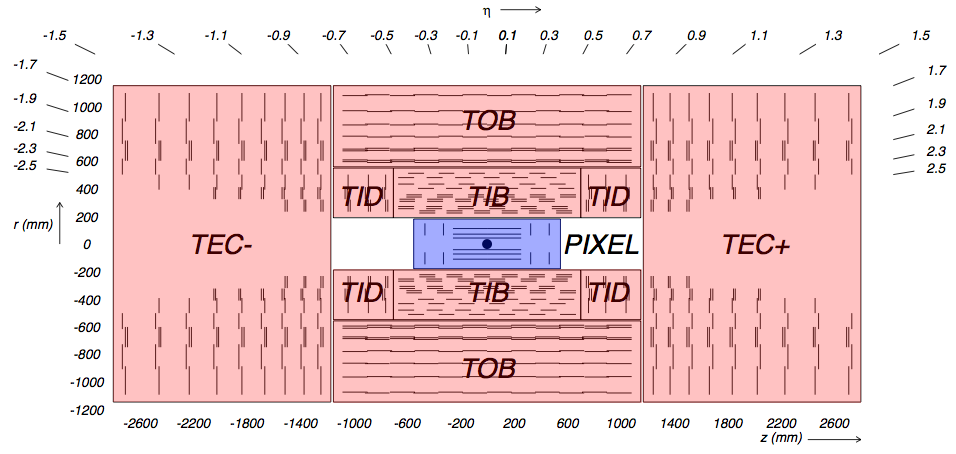
\includegraphics[width=0.75\textwidth]{figuras/Chapter2/Tracker.png}
      \caption{Layout of the Tracker System detectors. The blue part represents 
      the Pixel Detector and the red part represents the Strip Tracker: TIB,
      TID, TOB and TEC. Taken from \cite{chp2:CMS}.} \label{figchp2:Tracker}
    \end{center}
 \end{figure}

\textbf{Particle interaction with the Tracker material} \\

\noindent When a particle passes through the Tracker System it interacts not only with the active volume
of the detector, but also with the other components such as the read-out electronic, 
the mechanical structure, the services and the cooling system. This amount material is significant
and the interaction with the crossing particles must be considered. Figure \ref{figchp2:Tracker_TrackerMaterial}
shows the thickness (in terms of number of radiation lengths) of tracker material that a particle must 
pass through before reaching the ECAL. As a result, there is a high probability that 
photons, coming from $\pi^{0} \rightarrow \gamma\gamma$, can convert into electron-positron 
pairs which, as mentioned above, is important for jet and tau reconstruction.

\begin{figure}[ht]
    \begin{center}
      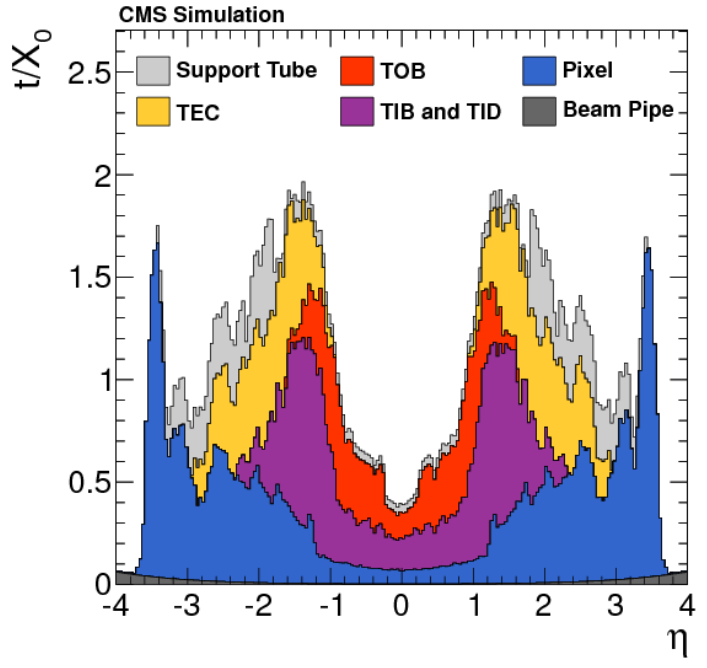
\includegraphics[width=0.45\textwidth]{figuras/Chapter2/Tracker_Thickness.png}
      \caption{The total Tracker material thickness (t) in units of radiation length X$_{0}$, as a 
      function of $\eta$. Taken from \cite{TrackerPerformace}.
      } \label{figchp2:Tracker_TrackerMaterial}
    \end{center}
 \end{figure}

\section{The Calorimeter System}

\noindent The purpose of the Calorimeter System is to stop most of the particles 
coming out from the collision and to measure their energy with a good 
granularity. Electrons, photons, and hadrons interact with the calorimeter 
material, depositing all their energy on the detectors which is sampled
and measured. The only SM particles that scape from the Calorimeter System are 
muons and neutrinos: muons deposit a very low amount of energy in this system, and 
continue traveling beyond to the detectors installed in the outer part of CMS, 
designed to reconstruct their tracks. In the case of neutrinos, they escape without detection
since they only interact weakly, leaving an energy imbalance in the event; therefore, this imbalance 
is an indirect evidence of their presence or the presence of any particle that only interacts weakly \footnote[1]{A big amount of energy 
imbalance would be an evidence of dark matter candidates, since they only participate on weak interactions.}. \\

\noindent The CMS Calorimeter is divided in two subsystems: the electromagnetic calorimeter (ECAL) and 
the hadronic calorimeter (HCAL). The ECAL is the closest calorimeter subsystem to the interaction point; 
it is designed to measure the energy of electrons and photons. The reconstruction of these particles 
is essential for many physics analyses, for instance for those in which 
jets or taus are involved. In these analyses, the photon and electron 
reconstruction is crucial for the energy measurement of the jet and for 
the tau identification. The HCAL, the other calorimeter subsystem, which is located 
just outside of the ECAL, is designed to measure the energy of the hadrons. It plays a fundamental
role in jet-like objects: QCD jets, b-jets, tau-jets; being able able to differentiate 
among these objects is crucial, is crucial, in particular for these analyses. Figure \ref{figchp2:CMStrajectories} 
shows the arrangement of the Calorimeter System and the energy deposits of SM particles on it.


%a jet contains a copious amount of 
%neutral pions which most of the times decays into one photon pair; since
%these photons might convert into electron-positron, the electron and 
%photon reconstruction is important for the energy measurement of the jet. Similarly, their
%reconstruction is important for tau identification since neutral pions are one of the decay 
%products of the tau-lepton. 

%because photons, that come from $\pi^{0}$ 
%decays ($\pi^{0}\rightarrow\gamma\gamma$), can convert into electron-positron pair; therefore, their 
%reconstruction is important for jet and tau identification, considering that $\pi^{0}$'s are produced copiously in 
%QCD jets and they are one of the tau decay products. 

%the granularity of the calorimeter is good enough to associate 
%the energy deposits of a charged particle with its reconstructed track on the 
%Tracker System

\subsection{The Electromagnetic Calorimeter}
\label{subsec:ECal}

\noindent The Electromagnetic Calorimeter is designed to absorb the total energy 
of electrons and photons when they pass through it. The interaction between these 
particles and the calorimeter material produces a cascade of electrons and photons in a process 
called electromagnetic shower. An electromagnetic shower starts when an energetic electron, 
or photon, enters into the high density medium of the calorimeter and starts to lose energy
due to interactions with the medium. Electrons and 
positrons lose their energy by bremsstrahlung radiation, while photons 
lose their energy by electron-positron conversions. Therefore, a cascade
of secondary particles is created and the energy losses continue through 
these two processes until the energy of the particles is not
enough to produce new ones. As a result, the energy deposits of the electromagnetic shower 
are spread over the calorimeter material and are sampled and measure using scintillators. The
 profile (transverse and longitudinal) of the electromagnetic shower allows to 
determine the energy of the incoming particle. Electromagnetic showers 
are then described by two parameters which depend on the calorimeter 
material: the radiation length (X$_{0}$) and the Moli\`ere radius. The radiation length is 
the distance than an electron or photon travels until its energy is reduced by a factor 
of $1/e$, while the Moli\`ere radius is the radius of a cylinder where 90$\%$ of 
the electromagnetic shower is contained. In consequence, the calorimeter 
is designed with enough thickness (in terms of radiation lengths) to measure the total
energy of the particles, and with a Moli\`ere radius small enough to achieve a good granularity. 
The schematic view of an electromagnetic shower is shown in Figure \ref{figchp2:EMshower}. 


%for pair production and the energy losses of electrons are dominated by other processes 
%than bremsstrahlung

\begin{figure}[ht]
    \begin{center}
      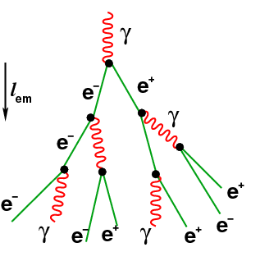
\includegraphics[width=0.3\textwidth]{figuras/Chapter2/ElectroCascade.png}
      \caption{Schematic view of the development of an electromagnetic shower. Taken from \cite{EMFigure}.
      } \label{figchp2:EMshower}
    \end{center}
 \end{figure}

\noindent The CMS ECAL has cylindrical and hermetic design with scintillators made of 
lead tungstate crystals (PbWO$_{4}$), see Figure \ref{figchp2:ECALcrytal}. The PbWO$_{4}$ crystals are
characterized by its high density (8.28 g/cm$^{3}$), its short radiation length (0.89 cm) and its
small Moli\`ere radius (2.2 cm), making them appropriate to achieve 
accurate energy measurements with a good granularity \cite{chp2:CMS}; additionally,
these crystals have excellent radiation-hardness and have a fast response, which make them
suitable for the LHC environment. When electrons or photons cross these crystals, they emit a light pulse 
with a time response of $\sim$25 ns (about 80$\%$ of the times). The scintillator
light is collected by photo-detectors that convert it into an electric signal. The photo-detectors 
used in the barrel are Avalanche Photo-Diodes (APDs) while in the endcaps are Vacuum Photo-Triodes (VPT). \\

\begin{figure}[ht]
    \begin{center}
      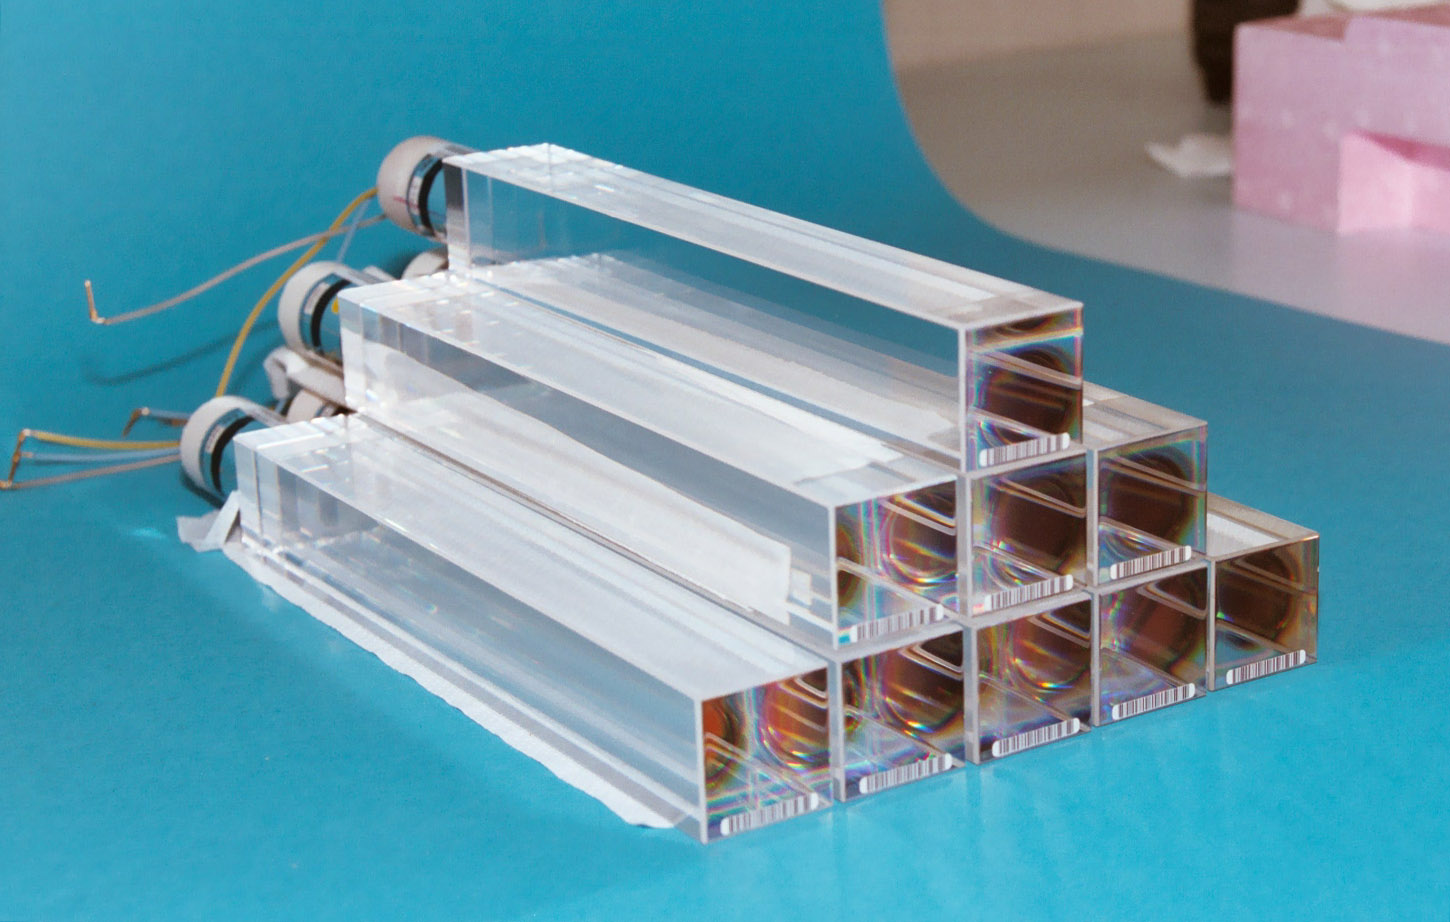
\includegraphics[width=0.33\textwidth]{figuras/Chapter2/ECALcrytal.jpg}
      \caption{CMS ECAL Lead Tungstate Crystals (PbWO$_{4}$).
      } \label{figchp2:ECALcrytal}
    \end{center}
 \end{figure}
 
\noindent The ECAL has 61200 crystals in the barrel and 7324 crystals in each endcap \cite{chp2:CMSTDR}, covering a 
$|\eta|$ range up to 3. The crystals are installed in a quasi-projective geometry 
in such a way that each of them points toward the center of the detector, plus an additional angle
of 3$^{\circ}$, with the purpose of avoiding particles passing through inactive regions of the ECAL. In the 
particles passing through inactive regions. In the barrel region, the calorimeter (ECAL Barrel or EB) has a 
inner radius of 129 cm, covering a pseudorapidity region of $|\eta| < $1.479. The EB crystals 
are 230 mm long (25.8 $X_{0}$) and cover a cross-section at the front face of 0.0174 $\times$ 0.0174 
in the $\eta-\phi$ plane (which corresponds to $22\times22$ mm$^{2}$). In the forward region,
the ECAL Endcaps (EE) are located at 314 cm from the collision point, covering a pseudorapidity range of
1,479 $ < |\eta| < $ 3,0. The EE crystals are 220 mm long (24.7 $X_{0}$) and cover
a cross-section of 28.62 $\times$ 28.62 mm$^{2}$. In addition to the crystals, \textit{Preshower Detectors}
are installed in front of endcaps, covering a pseudorapidity range of  $1.65<|\eta|<2.6$. This detector consists of two 
lead layers, each one followed by silicon sensors. Their main goal is 
to identify the two photons produced by neutral-pion decays in the
forward region. The complete ECAL arrangement is shown in Figure \ref{figchp2:ECAL}.

%with respect to this direction \footnote[1]{In the case of the endcaps, this angle 
%varies from 2$^{\circ}$  to 8$^{\circ}$.}; the purpose of this 
%geometrical arrangement is to avoid 


\begin{center}
\begin{figure}[h]
\centering
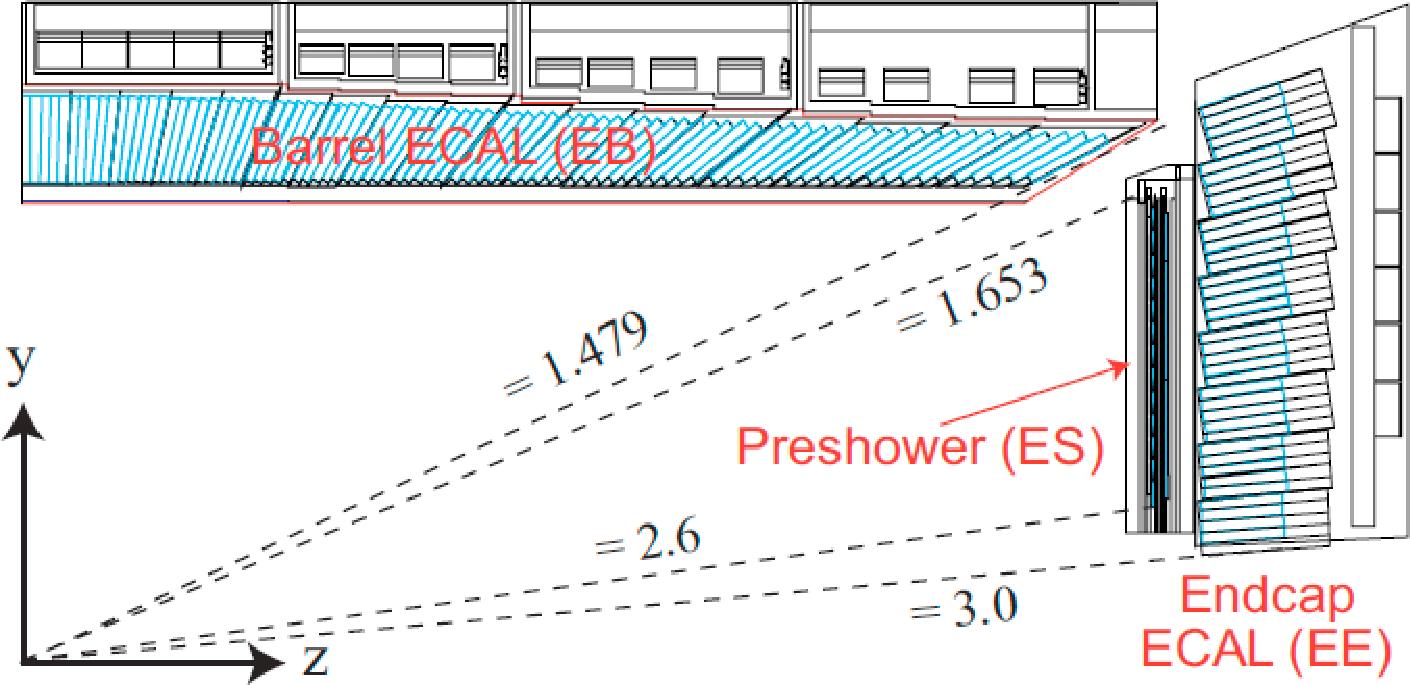
\includegraphics[scale=0.38]{figuras/Chapter2/ECAL.pdf}
\caption{Arrangement of the ECAL components.}\label{figchp2:ECAL}
\end{figure}
\end{center}

\noindent The energy resolution reached by the ECAL is given by:
\begin{equation} \label{ECALenergyResolution}
 \left(\frac{\sigma_{E}}{E}\right)^{2} = \left(\frac{2.8\%}{\sqrt{E}}\right)^{2} + \left(\frac{0.12\%}{E}\right)^{2} + \left(0.3\% \right)^{2} \;, 
\end{equation}

\noindent where the first term comes from the stochastic nature of electromagnetic showers, the second term is 
related to electronic noise and the third term is related to the systematic uncertainty produced 
by the calibration of the apparatus. As can be inferred from
Eq. \ref{ECALenergyResolution}, the energy resolution for energetic particles is dominated by the systematic uncertainty, while
the stochastic and noise terms are dominant for low energies. As an example, the energy resolution 
obtained in the EB is close to 1$\%$ for all electrons that come from Z decays \cite{ECALperformance}.

\subsection{The Hadronic Calorimeter}
\label{subsec:HCal}

\noindent The Hadron Calorimeter (HCAL) is designed to stop the hadrons and to measure 
their energy. It is composed of fluorescent scintillators inserted in layers of 
a dense material called the absorber. The absorber is made of stainless 
steel and copper layers. When a hadron hits the absorber it produces a cascade of 
particles, known as hadronic shower. The hadronic shower is a cascade of 
secondary particles, mainly pions, originated by strong interactions between 
the hadron and the atomic nuclei of the absorber material. Due to copious pion
production, the shower also acquires electromagnetic components through
neutral pion decays into photons. As the hadronic shower develops, the particles 
are detected by the scintillators, producing light pulses that are collected by 
optical fibers. The amount of light collected is proportional to the amount 
 of energy deposited in the scintillator material, allowing the energy to be measured. A hadronic 
 shower is described by the absorption length, which is the average distance traveled by the 
 hadron trough the medium before it interacts with the absorber; it is given by:

 \begin{equation}
 \lambda = \frac{A}{N_{A} \sigma_{abs}}  \;,
\end{equation}

\noindent where $A$ is the nuclei weight, $N_{A}$ is the Avogadro's number and $\sigma_{abs}$
is the absorption cross-section.\\

\noindent In the central pseudorapidity region (HCAL Barrel, HB) the volume
is restricted due to the solenoid, for this reason, part of the calorimeter is installed 
outside (Hadron Outer Calorimeter, HO) to achieve the desired level of the hermeticity. In 
the forward region there are two subsystems installed: the HCAL Endcaps (HE) 
which cover the pseudorapidity range of 1.4 $< |\eta| <$ 3; and the HCAL Forward (HF) which 
extends the $\eta$ coverage up to 5.2. The HCAL structure is shown in Figure \ref{figchp2:HCAL}.

%3$ < |\eta| < $5.2.


\begin{center}
\begin{figure}[h]
\centering
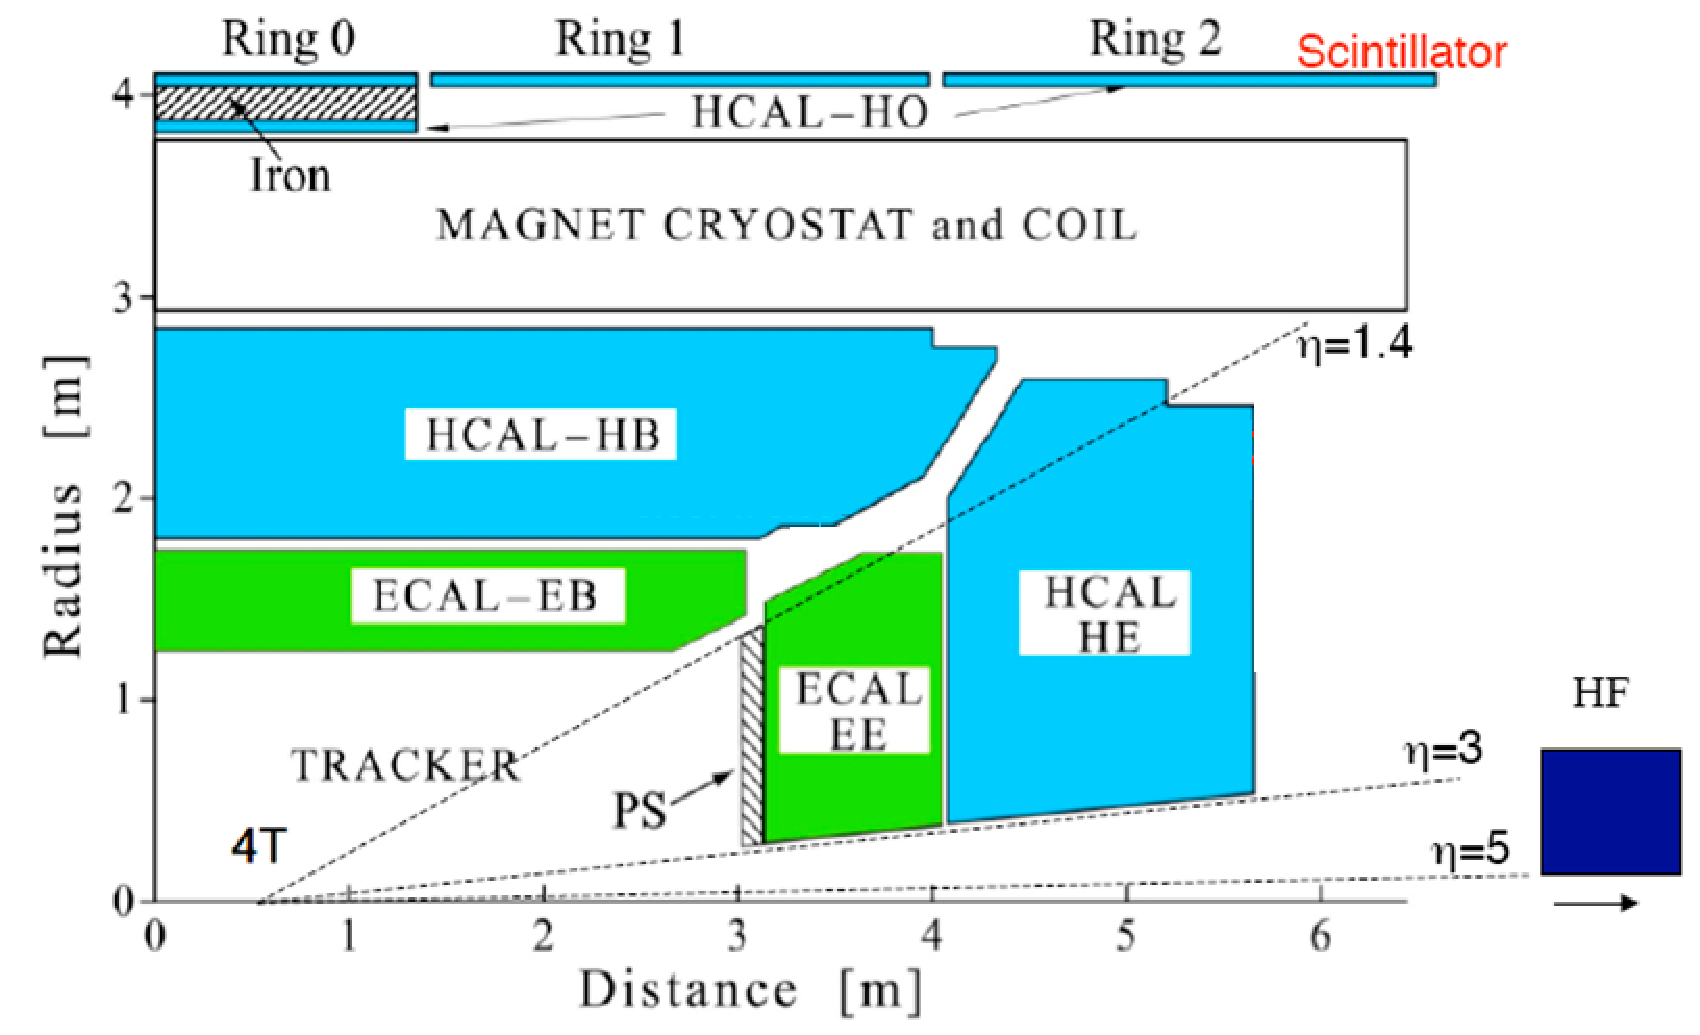
\includegraphics[scale=0.4]{figuras/Chapter2/HCAL1}
\caption{Disposition of the HCAL components.}\label{figchp2:HCAL}
\end{figure}
\end{center}

\noindent The HB is divided into two identical halves in the $z$-direction. Each half is composed of 18
wedges, covering a range of $|\eta| < $ 1.4. Each wedge consists of brass absorber plates 
staggered with plastic scintillators. The brass is a non-magnetic material and it has a 
small radiation length ($\lambda = $ 16.42 cm), making it appropriate for the CMS environment. Between every
two layers of absorbers, there is plastic scintillator with a thickness of 3.7 mm; the scintillator 
sends lights pulse through optical-fibers (WaveLenght Shifter, WLS) to the
photo-detectors (Hibryd Photodiodes, HPD). The photo-detectors convert the light 
into an electric signal. The innermost and outermost plates of 
the wedge are made of stainless steel in order to strengthen the structure. Each wedge 
is segmented in the $\eta$-direction by 16 structures called towers; each tower 
covers an identical solid angle whose area in the $\phi-\eta$ plane is 0,087$\times$0,087. \\

\noindent The HO is located outside the solenoid, covering $|\eta| < $ 1.26. It uses as absorber 
material the solenoid itself and the inner most layer of the iron-yoke structure. The HO 
is divided into 5 wheels in the $z$-direction, similar to the geometrical disposition 
of the Muon Chambers (see Section \ref{sec:MuonSys}). In the central wheel of the detector, there 
are two layers of plastic scintillators staggered between the solenoid and the inner 
layer of the iron yoke. Additionally, there is one scintillator installed in 
each remaining wheel just behind the solenoid. Figure \ref{figchp2:HCAL} shows the disposition of 
the HO plastic scintillators. \\

\noindent The HE is a sampling detector similar to the HB, composed of brass layers 
staggered with plastic scintillators of 3.7 mm of thickness. The HF 
is located at 11.2 m from the interaction point in the $z$-direction,
covering an extended $\eta$ region up to 5. The purpose of the HF is 
to achieve a better hermeticity, which improves the reconstruction of very forward 
jets as well as the measurement of the energy imbalance of the event. \\

\noindent Due to the nature of a sampling detector like the HCAL, its energy resolution 
is worse than the one obtained by the ECAL. For example, for pion it is \cite{chp2:CMS}:

\begin{equation} \label{CALResolution}
 \left(\frac{\sigma_{E}}{E}\right)^{2} = \left(\frac{138\%}{\sqrt{E}}\right)^{2} + \left(13\% \right)^{2} \;.
\end{equation}

\noindent Although the HCAL does not provide a high energy resolution, it is not crucial
since this information is combined with the one of other detector systems.

\section{The Muon System}
\label{sec:MuonSys}

\noindent The purpose of the Muon System is to identify and reconstruct muons but also,
to generate trigger signal for the data acquisition system. This system
is located outside the solenoid since the muons are the only known charged particles 
than can cross the tracker, the calorimeters and the solenoid material. In order to achieve the
muon reconstruction and to trigger with them, CMS has three different kinds of 
Muon Detectors: Drift Tubes (DTs) in the barrel, Cathode Strip Chambers (CSCs) in endcaps and Resistive 
Plate Chambers (RPCs) in both, in the barrel and the endcaps. The DTs and the CSCs are used for tracking 
purposes. The RPCs are used for triggering due to their high time 
resolution. The Muon System structure is shown in Figure \ref{figchp2:MuonSystem}. In summary, 
the three technologies used in the Muon Chambers are:

\begin{itemize} 
 \item \textbf{Drift Tubes}, or DTs, are gaseous detectors used for tracking due to their excellent spatial resolution.
The DT basic cell is a tube filled with a gas mixture of 85$\%$ Ar and 15$\%$ CO$_{2}$.
The anode is an aluminum wire placed longitudinally in the center of the tube.
The tube has a cross section of 13 $\times$ 22 mm$^{2}$ and a length between 2 to 3 m,
depending on to the position of the chamber in the barrel. When a charged particle passes through the cell 
the gas is ionized and produces an avalanche of electrons, because of the high 
electric field close to the wire. The signal deposited by the electrons in the wire is later amplified. 
 \item \textbf{Cathode Strip Chambers}, or CSCs, perform the muon track reconstruction in the endcaps. Each CSC chamber
has a trapezoidal shape in order to cover the 12 azimuthal sectors of the detector. A CSC Chamber 
has 6 planes of wires along the azimuthal direction, defining the radial coordinate of the track. The wire
planes are intercalated with 7 panels of cathode strips that run radially and give the $\phi$ measurement 
with a resolution of 10 mrad. There are a total of 540 CSCs in the CMS detector. %, where 72 new Chambers installed in the forth disk during the LS1. 
\item \textbf{Resistive Plate Chambers}, or RPCs, are gaseous parallel-plate detectors 
with a time resolution of about 1 ns. These detectors have an important roll for the triggering
system, since they have excellent time resolution suitable for the identification of the BX 
associated to the detected muon. There are 6 RPC layers in the barrel
and 4 disks in each endcap (see Figure \ref{figchp2:MuonSystem}). 
 \end{itemize}


\begin{center}
\begin{figure}[h]
\centering
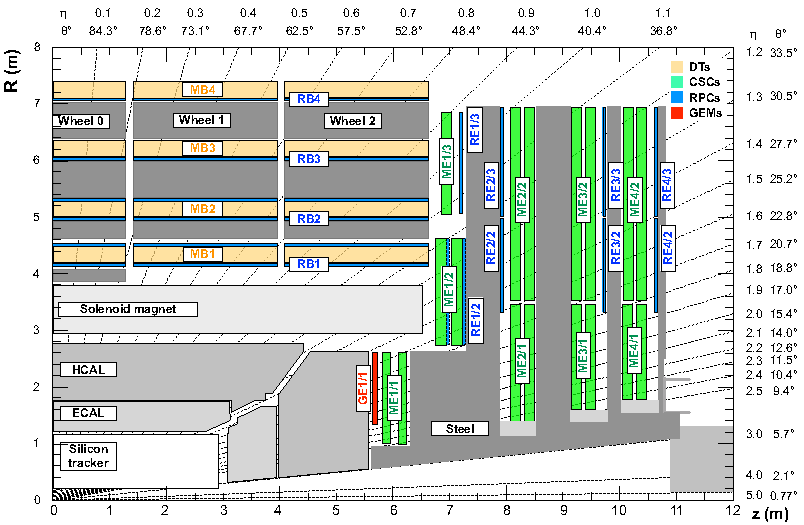
\includegraphics[scale=0.4]{figuras/Chapter2/MuonSystem}
\caption{Longitudinal view of CMS, showing the Muon System layout: DT Detectors are represented in pink,
CSCs are green and RPCs are blue. GEM Detectors, that will be installed in LS2, are in red.}\label{figchp2:MuonSystem}
\end{figure}
\end{center}

\noindent In the barrel region, the Muon Chambers (DTs and RPCs) are inserted into the 
five wheels of the iron yoke; they form four concentric cylindrical 
layers, each of them divided on 12 sectors in $\phi$. Then, the geometrical 
arrangement of the Muon System consists on 5 wheels in the $z$-direction, 4 layers in 
the $r-$direction and 12 sectors in the $\phi-$direction. In the forward region, the Muon 
Chambers (CSCs and RPCs) are arranged into 4 disks in each endcap , where each disk is 
divided into 12 sectors in the $\phi-$direction and 4 rings in the $r-$direction. \\

\noindent The use of two types of detectors, DTs and RPCs in the barrel and CSCs and RPCs in the endcap
improve the muon reconstruction resolution and efficiency. The RPCs provides a fast 
response ($<$ 25 ns), allowing the identification of the BX, while the DTs and CSCs provide 
a high spatial resolution. The information obtained from the Muon Chambers
is combined with the one provided by the Tracker system in order to 
improve the muon identification efficiency and the muon reconstruction. For instance,
the momentum resolution for muons of \pt~$= 10$ \GeV~ is 10$\%$ using only the Muon Chambers information
, while it becomes 1$\%$ when it is combined with the Tracker System information\cite{chp2:CMSTDR}.\\

\noindent During the Long Shut Down 2 schedule to 2019 (LS2) Gas Electron Multipliers (GEMs) will be installed in 
the endcaps in order to improve the muon identification efficiency and the momentum resolution in 
these regions (see Figure \ref{figchp2:MuonSystem}). In addition to their 
high granularity, GEMs will be used for triggering, due to their high time resolution.

\section{The Trigger and Data Acquisition Systems}
\label{sec:Trigger}

\noindent The Trigger and the Data Acquisition (DAQ) Systems use the information 
provided by the Tracker, the Calorimeter, and the Muon Systems in order 
to identify the events with interesting physics and to store them to be 
analyzed afterwards. The information of an event is stored in 
the read-out electronics of each sub-detector system; when these 
pieces are combined, the data size of an event is around 
1 MB (1 MB per BX). Considering that the LHC 
operates with a collision rate of 40 MHz at nominal luminosity, CMS could 
deliver up to 40 TB of information per second. The data storage 
for such high rate is impossible with the current technology, but also only the hard
scattering collisions (interesting events) should be selected and stored. These collisions
happen very seldom, in consequence, the Trigger System is used to 
select only those events, reducing the rate from 40 MHz to 100 Hz, and making 
it feasible to store that data using the Data Acquisition System (DAQ).

%The read-out electronics of each sub-detector can 
%keep stored the information only for 3.2 $\mu$s before it is erased,
%therefore they receive an electric signal from the Trigger System in order to 
%deliver the event information to processor. Additionally, while the 
%Trigger System is deciding if the event is selected or discarded, the 
%read-out electronics must keep storing the information of the subsequent collisions. 


\subsection{The Trigger System}
\label{subsec:Trigger}

\noindent The Trigger System performs the selection of the hard scattering events in two steps:
the Level-1 Trigger (L1 Trigger) and the High Level Trigger (HLT). The first step, the Level-1 Trigger,
is performed by programmable read-out electronics in order to reduce the event rate from 40 MHz 
to 100 kHz. The second step, the HLT, is performed by about one thousand processors, which through
software algorithms reduce the event rate up to 100 Hz. \\

\textbf{The Level-1 Trigger}\\

\noindent The Level-1 Trigger performs the first event selection through hardware criteria programmed 
in the read-out electronics of each sub-detector. A hard scattering event typically 
involves heavy particle production such as b-quarks, t-quarks, heavy bosons 
or hight-\pt~muons; then, interesting physics events usually contain high \pt~jets and muon signals. In 
consequence, the Level-1 Trigger searches for signals into the read-out electronics 
of the Calorimeter System and the Muon System. The information provided by these two sub-detectors
is combined and sent to the Global Trigger System; this system decides
if the event is accepted sending a signal, known as \textit{L1-Accept}, to the read-out electronics, so that
it stores the information of the event \footnote[1]{If the L1-Accept signal is not produced for an event, the data associated to that event is 
erased from the readout electronics memory.}. Once the event is stored by the DAQ System, the data is moved 
to the HLT, where a second level of triggering is performed. Figure \ref{figchp2:TriggerSystem} shows 
the data flux through the L1 Trigger System. \\

\begin{center}
\begin{figure}[h]
\centering
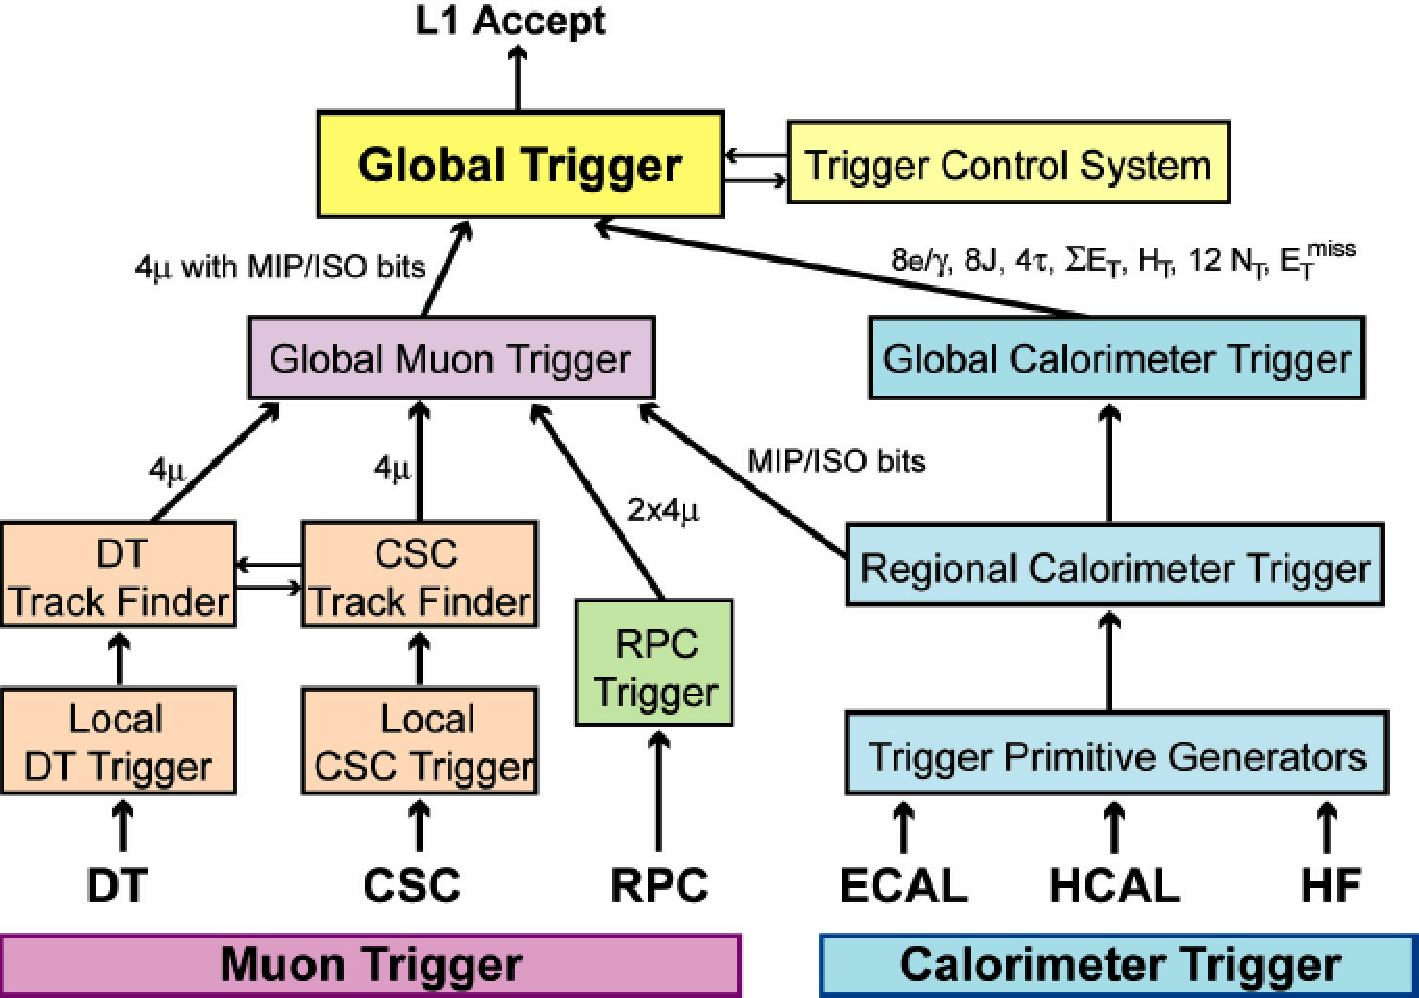
\includegraphics[scale=0.35]{figuras/Chapter2/trigger}
\caption{The Level-1 Trigger architecture. The L1-Accept signal is produced when 
the event passes the three trigger component criteria: local, regional and global.}\label{figchp2:TriggerSystem}
\end{figure}
\end{center}

\textbf{The High Level Trigger}\\

\noindent As mentioned above, the events selected by 
the L1 Trigger are delivered to a farm of about one thousand 
processors, where the High Level Trigger is executed. Unlike 
the L1 Trigger, which is implemented in hardware, the 
HLT selection is implemented in software since more 
complex algorithms are applied. The selection performed by the 
HLT starts with the readout of the information coming 
from each sub-detector system; then, the
processors apply algorithms to the data in order to perform a quick 
reconstruction of the physics objects in the event; finally, the
hard scattering events are identified. The events that pass 
the HLT trigger, about 100 events per second, are stored in disk. The stored data 
is labeled according to the physics objects identified on each event; for 
instance the triggered events due to the presence of a muon are 
labeled as \textit{SingleMuon} dataset, and hence analyses which involves muons in the final state 
only use  the muon dataset instead of all the dataset stored by CMS.


%the collected data is moved to
%on-line servers with the purpose of studying the CMS performance, in a process known as Data Quality
%Monitoring or DQM. 




\subsection{Data Acquisition System}
\label{subsec:Trigger}

\noindent The Data Acquisition System (DAQ) stores the events selected by the Trigger System. Since 
the read-out electronics of each sub-detector can store the information of an event 
only for 3.2 $\mu$s, the data will be erased unless a L1-Accept signal is received before 
that time. However, while the Trigger System is deciding if the event is selected or discarded, the 
read-out electronics must keep storing the information of the subsequent collisions; for 
this purpose electronic devices known as Front End Systems (FES) are used, which store data continuously 
in 40-MHz pipelined buffers. Once the L1-Accept signal reaches the FES, the 
data is pushed into the DAQ system via Front End Driver devices (FED). The DAQ System
uses Front-end Read-out Link devices (FRL) in order to combine the information provided 
by several FEDs of each sub-detector, resulting in a data file suitable for the HLT processing. Finally,
the event information is delivered to the farm of processors through optical links, where the HLT
trigger is applied. The DAQ system is designed to operate with same input frequency 
than the L1 Trigger and to deliver data to the HLT System.


%therefore they receive an electric signal from the Trigger System in order to 
%deliver the event information to processor. Additionally, while the 
%Trigger System is deciding if the event is selected or discarded, the 
%read-out electronics must keep storing the information of the subsequent collisions. 
  

%this information includes, for example, the BX 
%of the collision from which the detected signal comes, the position
%in the detector, etc. This information provided by several FEDs arrives to the 
%Front-end Read-out Link (FRL) and finally they are delivered to the 
%farm of processors through optical links, where the event information 
%is processed by the HLT. 

\subsection{Data Processing}
\label{chap2:dataprocessing}

\noindent The data recorded by the DAQ system results in a data file which contains all the information for
the accepted events. The data delivered by the HLT have a RAW format, which is not
suitable for physics analysis; therefore a reconstruction process is performed on it in 
order to identify all the physics objects and determining their kinematics variables. CMS uses 
the Particle Flow algorithm in order to reconstruct every particle coming from the pp collision; the 
Particle Flow algorithm and the particle reconstruction are described 
in Chapter \ref{chap:ParticleID}. As a result, the reconstructed physics objects are stored in a RECO data 
format; nevertheless, the RECO data is still not appropriate for physics analysis due to its large 
storage size on disk. Hence, two skimming processes are performed on the RECO data, resulting in 
a data file known as mini-AOD. The mini-AOD contains only the relevant information 
of the physics objects, making them appropriate for physics analysis. \\



%There are several stages from the pp collision to the data analysis. 
%After the pp collision produced by the LHC, all the particles coming out from interaction
%are detected by the CMS Detector Systems. Then, the Trigger and the DAQ Systems select and 
%store the interesting events, resulting in a data 

%file which contains all the information of 
%the event. 


%This Chapter has shown the process from the production of pp 
%collisions by the LHC: the detection of the products of a collision by 
%the CMS detector systems, the selection and the storage of the interesting 
%events by the Trigger and DAQ systems. 


%The full data are stored in pipelined-memories of processing elements, while waiting for the trigger decision.
%rigger latency, between a given bunch crossing and the distribution of the trigger decision to the
%detector front-end electronics, is 3.2 μs [91][14]. 

%The full data are stored in pipelined-memories of processing elements, while waiting for the trigger decision.
%rigger latency, between a given bunch crossing and the distribution of the trigger decision to the
%detector front-end electronics, is 3.2 μs [91][14]. 

%A schematic view of the components of the CMS DAQ system is shown in figure 9.2. The
%various sub-detector front-end systems (FES) store data continuously in 40-MHz pipelined buffers.
%Upon arrival of a synchronous L1 trigger (3.2 μs latency) via the Timing, Trigger and Control
%(TTC) system [204, 207], the corresponding data are extracted from the front-end buffers and
%pushed into the DAQ system by the Front-End Drivers (FEDs).





%Once the Trigger System identify an interesting event, a signal 
%is send to the read-out electronics in order 

%\subsection{Physics Objects}
%\label{subsec:PhysicsObjects}


